\documentclass[a4paper,11pt]{article}
\usepackage{graphicx}
\usepackage{enumerate}
\usepackage{caption}
\usepackage[usenames, dvipsnames]{color}
\usepackage[margin=1.25in]{geometry}

\begin{document}

\begin{flushright}

\vspace{1.1cm}

{\bf\Huge Apollo Guidance Computer}

\rule{0.25\linewidth}{0.5pt}
%\noindent\rule{\linewidth}{1.0pt}


\vspace{0.5cm}
%Put Authors
Justin Ely
\linebreak
\newline
%Put Author's affiliations
\footnotesize{605.411 Foundations of Computer Architecture \\}
\vspace{0.1cm}
% Date here below
6 December, 2016
\end{flushright}

\noindent\rule{\linewidth}{1.0pt}


%%%%%%%%%%%%%%%%%%%%%%%%%%%%%%%%%%%%%%%%%%%%%%%%%%%%%%%%%%

\section{Contents}
\begin{itemize}
\item Introduction and Overview %(page \pageref{sec:Introduction})
\item Data representation
\item Instruction Set
\item Memory
\item Summary
\item References
\end{itemize}

%%%%%%%%%%%%%%%%%%%%%%%%%%%%%%%%%%%%%%%%%%%%%%%%%%%%%%%%%%

\section{Introduction and Overview}

While the Apollo project was gaining steam in the 1960's, digital computing was yet in it's infancy.  This provided great opportunities for the space program; from drastic reductions in component size to exponential increases in the power of computing equipement.  However, as history has shown, the pace of advancement in digital computing has been incredibly rapid, and attempting to keep track can produce interesting results as both technology and mission requirements evolve through more than a decade of use.  

Both the Apollo Command Module and the Lunar Module utilized a computer called the Apollo Guidance Computer (AGC) for control of guidance and navigation.  This system controlled and facilitated activities like velocity and orientation corrections during spaceflight.  Astronauts would interface with the AGC through the Display and Keyboard interface (DSKY), which had it's own high-level language into the low-level AGC.  (MIT PDF)

\begin{figure}[h!]
\caption{Apollo Guidance Computer (AGC) {\it (left)} next to the DSKY (Display and Keyboard) interface {\it (right)}.} 
\centering
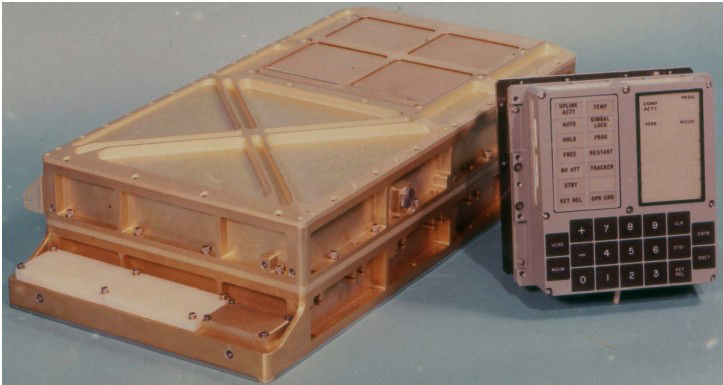
\includegraphics[width=.8\textwidth]{Agc_view.jpg} 
\end{figure}
\vspace{0.02cm}

Created by the Charles Stark Draper Laboratory and fabricated by Raytheon, the AGC was a modest 12.5x13x6 inches in size but weighed an impressive 70 pounds.  It's power consumption was comparable to a modern laptop at approx 55 watts.  (Wikipedia)  The APG was designed around a Von Neumann Architecture with a CISC instruction set architecture and only integer arithmetic units.  The Von Neumann design, where both instructions and data occupied the same memory, served to simplify the hardware and control system. (MIT PDF) The exclusion of floating point units also helped for simplicity and fabrication, but at the cost of complexity in the representation of real numbers.  

The memory system had a total of 38K words in a flat namespace of registers, writable memeory, and read-only memory (ROM).  Each wod was 16 bits, though the first bit dedicated to parity and unaccessible to the programmer.  The APG is also a one-address machine, where instructions specify only a single register or memory location.  The other register is always assumed, typically the general-purpose accumulator for the logical and arithmetic operations, but also specific registers for memory, interrupts, or temporary storage.  This served to shorten and simplify commands when memory was at a premium, and permit the same calculations with fewer registers at a time when they were difficult to manufacture.  

This paper goes into detail into some of the more unique characteristics of the APG which highlight the technical difficulties faced in the early era of computing.  The data representation illustrates trade-offs between feasibility and desireability, the instruction set shows how fortunate we are to have large word sizes, and the memory system can be most easily contrasted with current systems to see the advancement of technology.  

%%%%%%%%%%%%%%%%%%%%%%%%%%%%%%%%%%%%%%%%%%%%%%%%%%%%%%%%%%

\section{Data Representation}
The data representation scheme used in the APG was a direct result of balancing the speed and efficiency of small word sizes against the accuracy of calculations.  Though a large word size has the benefit of providing much better precision to numerical values, it also requires larger registers, wider buses, and more system memory.  During this period, none of these were at a premium, and so sacrifices in precision had to be made.  However, these sacrifices couldn't get in the way of mission success, where inaccuracy could mean the difference between landing and crash landing.  In the end, engineers concluded that a word size of 15 bits, 16 counting the parity bit which is ignored in the following sections, was a sufficient size for instructions and provided enough precision for the equations used in navigation and control. This would allow double-precision values of 28 bits to give approximately 9 decimal digits of precision.  This amount of precision translated into distances of about 1 foot and velocities below 1 foot per second.  

\subsection{Integers}
The APG represents integers using a modified version of one's complement. As in the standard implimentation, the first bit is used for the sign with the remaining 14 bits dedicated to the value.  This allowed representation of values from -16383 to 16383 including both positive and negative zeros. 

The modification to the standard one's compliment is specifically to handle overflow by adding special detection of sign bit flips.  When performing calculations, the 15 bit value is loaded into a 16-bit accumulator, where the 16th bit is a copy of the sign bit from the operand.  If the result of an operation unexpectantly changed the sign of the output, the AGC would automatically detect that overflow had occured and would alter the program by temporarily halting all interrupts.  This was a level of protection against other system programs using the incorrect result of the calculation.

The suspension of interrupts could be cleared by many actions, such as loading a completely new value into the accumulator, after which normal operation would resume.  Additionally, when overflow has occured and the result is saved, the {\it original} sign is saved instead of the computed one.  This has the strange behavior of returning a number with an incorrect magnitude, but correct sign.  This is just another protection in a system that needed to be incredibly fault tolerant; keeping values in the expected range may prevent hard-to-debug errors down the line from sign-flipping results.

\subsection{Real Numbers}
Real numbers were incredibly important in the sort of mathematical calculations that the APG needed to perform in it's routine operations.  From the inputs and results of calculations, to mathematical constants like the location of guidance stars and PI.  However, with only integer units, the APG had no native ability for representing or performing arithmetic on floating point numbers.   Instead, an alternative system was used to do calculations on real numbers called fractional notation.

\begin{figure}[h!]
\caption{Integer and Fractional number representation in the AGC.} 
\centering
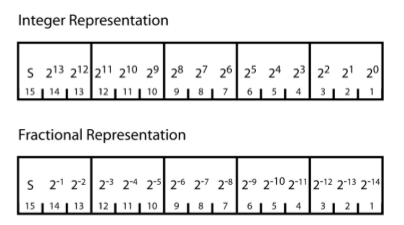
\includegraphics[width=.8\textwidth]{apg_numbers.png} 
\end{figure}
\vspace{0.02cm}

In this system, every bit in the word represents negative powers of 2 as shown in Figure 2.  With this system, real numbers could be represented and manipulated without the need for floating point hardware.  However, this system has a serious flaw; it completely lacks any order of magnitude and can only represent numbers between 0 and 1.

This constraint put a huge burden on programmer to know the data that would pass through a system incredibly well and to safeguard for exceptions.  Values used in a program needed to be arranged to only require a single order of magnitude at a time.

\subsection{Units}
An interesting side-note concerns the mathematical units used in the computations.  Internally to the APG, the units were metric.  However, the astronauts wanted to read and input values in Imperial, so conversions were employed in the layer between the core and the UI. 

%%%%%%%%%%%%%%%%%%%%%%%%%%%%%%%%%%%%%%%%%%%%%%%%%%%%%%%%%%

\section{Instruction Set}
The APG is a Complex Instruction Set Computer (CISC), where instructions perform complex tasks through microprogrammed implementations requiring many clock cycles.  This is clearly evident in many of the available commands, such as ADS which performs addition into a memory location.  This behavior is in stark contrast to a Reduced Instruction Set Computer (RISC), where typically only Load and Store commands may access memory.  

The basic format for instructions in the AGC is shown in the diagram below.  The first bit provides parity, the next 3 bits are the op-code, and the remainder is the operand or address.  A mostly complete list of commands can be seen in Table 1 below.

\begin{center}
\begin{tabular}{| c | c | c |}
  \hline	
  	Parity & Op-code & Address \\ \hline \hline
	1 & 011 & 0001 1010 1110 \\ \hline
\end{tabular} \\
\captionof{table}{Example instruction showing field breakdown.}
\end{center}

A 3-bit opcode allows for a total of only 8 unique instructions.  Clearly, trying to work the entire operation of a complicated spacecraft with only 8 instructions presents significant challenges.  Many more instructions became necessary as the mission requirements progressed, but it would have been too costly to re-design the system around a larger word size.  To bypass the limitations of the current system, the engineers created some unique solutions to get more instructions.

The first addition to the instruction set came from exploiting existing commands that could utilize smaller operand fields.  In particular, instructions that write to memory will never be able to write to ROM. Since ROM is the higher 36K words, these instructions would only ever address the first 2K words, and will only ever use the lower 10 bits of the operand field. By combining the two left-over bits, called quarter-codes, with the opcodes for this subset of commands yields an entirely new suite of available instructions.  This provided additional instructions by re-purposing the opcodes from TS, ADS, INCR, and XCH.

The quarter codes expanded the instruction set considerably, and added efficiency to the system by giving useful meaning to opcode/addresses combinations that wouldn't work with the memory system, but still more were needed.  To further add to the available commands, the engineers repurposed nonsensical (though technically valid) instructions.  One example of this would be using the TC command to transfer control to the EBANK register.  This register was only 3 bits wide and would never contain valid instructions or data, and so would serve no purpose.  Instead, the AGC turned TC to EBANK into a brand new instruction: RELINT (Enable Interrupts).  Similarly, this was done for TC commands to 3 other registers that would never be valid.  This strategy served not only to expand the available commands, but to also serve as protection against programmer error.  If TC to EBANK ever was accidently entered, without the protection of the special commanding, the effects could be very difficult to debug.

Lastly, when these commands still proved insufficient, a brute-force software solution was employed.  One of the special cases described above, TC to the BBANK register, was changed to instruct the AGC to interpret the subsequent command using an entirely new set of opcodes.  This effectively created a second instruction set, complete with quarter codes and special cases like in the original.  Though this nearly doubled the possible instruction set, it comes at the cost of increased software overhead to processing the extended set.  This was mitigated as much as possible by placing the most often used opcodes in the standard set, and the less-frequently used ones in the extended.

\begin{center}
\begin{tabular}{| c | c | c |}
  \hline	
  	Group & Command & Meaning \\ \hline \hline
	Sequence Changing & TC & Transfer Control \\ \hline
	& TCF & Transfer Control to Fixed \\ \hline
	& CCS & Count Compare and Skip \\ \hline
	& BZF & Branch Zero to Fixed \\ \hline
	& BZMF & Branch Zero or Minus to Fixed \\ \hline
	
	Reading and Writing & CA & Clear and Add \\ \hline
	& CS & Clear and Subtract \\ \hline
	& DCA & Double Clear and Add \\ \hline
	& DCS & Double Clear and Subtract \\ \hline
	& TS & Transfer to Storage \\ \hline
	& XCH & Exchange A and K \\ \hline
	& LXCH & Exchange L and K \\ \hline
	& QXCH & Exchange Q and K \\ \hline
	& DXCH & Double Exchange \\ \hline
	
	Arithmetic and Logic & AD & Add \\ \hline
	& Su & Subtract \\ \hline
	& ADS & Add to Storage \\ \hline
	& MSU & Modular Subtract \\ \hline
	& INCR & Increment \\ \hline
	& AUG & Augment \\ \hline
	& DIM & Diminish \\ \hline
	& DAS & Double Add to Storage \\ \hline
	& MASK & Mask A by K \\ \hline
	& MP & Multiply \\ \hline
	& DV & Divide \\ \hline

	I/O Channel & READ & READ KC \\ \hline
	& WRITE & Write Channel KC \\ \hline
	& RAND & Read and Mask \\ \hline
	& WAND & Write and Mask \\ \hline
	& ROR & Read and Superimpose \\ \hline
	& WOR & Write and Superimpose \\ \hline
	& RXOR & Read and Invert \\ \hline
	
\end{tabular} \\
\captionof{table}{Commands of the AGC broken up by section.  Some commands ommitted for brevity.}
\end{center}

%%%%%%%%%%%%%%%%%%%%%%%%%%%%%%%%%%%%%%%%%%%%%%%%%%%%%%%%%%

\section{Memory}
The memory system of the APG differs significantly from the systems we're accustomed to today.  Physically, three different memory structures were employed; flip-flops for registers, coincident current ferrite cores for writable memory, and fixed core rope for read-only memory (ROM).  These three structures were each optimized for there particular use case.  The use of magnetic memory was very important for space based applications as it was immune to most radiation-induced errors and would persist after the removal of the power source.

The writable ferrite-core memory was constructed as millimeter sized ferrite rings which stored 1's and 0's as magnetization in opposite directions.  This memory contained some programs, results, and temporary space.  

Magnetic core rope served as the ROM for the AGC, and contained copre operational programs, but also kept mathematical constants, like star locations, to prevent any overwrite operations.  These contents of were physically written during fabrication, which provided the enforcement of the read-only characteristic.  This memory was compact, reliable, had random access, and was extremely inexpensive.  Each bit cost between \$.05 and \$.07 to produce when most comparable solutions were a factor of 10 higher. (MIT) The main detractor to rope memory came from being programmed during fabrication.  This meant that any desired change, due to changing requirements or simple mistakes in programming or manufacture, couldn't be implemented without re-wiring the core.  Due to their complexity, this usually meant entire modules needed to be replaced for any change.  (MIT)

\begin{figure}[h!]
\caption{Schematic of core rope memory.} 
\centering
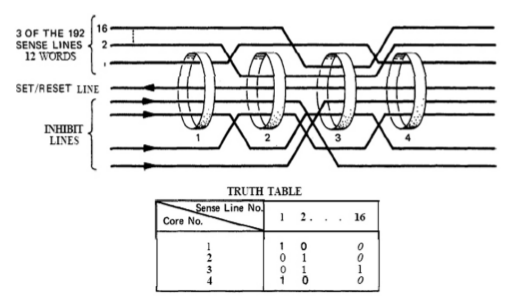
\includegraphics[width=.8\textwidth]{core_rope.png} 
\end{figure}
\vspace{0.02cm}

Of the 38K words in the total system memory, the first 48 words belonged to the central registers.  The next 2K were the writable memory, and the remaining 36K were ROM.  Furthering the departures from current trends, the registers were addressable just like the other memory locations.  This allowed the same instructions to be used for memory and register access, further simplifiying the system design.  

The 38K flat memory space, though convenient, posed a problem for the instruction set.  1 bit for parity and 3 bits for opcode left only 12 bits for calculation of the address in memory.  This was only sufficient to address about 4K of memory; far short of the 38K necessary.  At this time in history, memory was relatively cheap and allowed systems to have far more memory than was physically addressable with a reasonable word-size.  Contrast this today, where modern 64-bit word-sizes can address far more memory than can be included with the system.  Additionally, virtual memory management wasn't yet in a mature form at this time in computing history. 

To combat this, a "memory banking" scheme was used. The writable memory was divided into 8 banks of 256 words each.  Similarly, the ROM was divided into 36 banks of 1024 words each.  Instructions to writable memory would use the first two bits to select a bank, and the remaining 10 to select an offset in that bank.  Instructions to ROM were handled slightly differently depending on the access location.  Some locations low in address were able to be directly selected with the 12 bit address field.  For higher locations, selected by the contents of the 11th and 12th bits, the 10 lower bits are appended to the 5 bit contents of a special FBANK register to achive the necessary 15 bits of the address.  

%%%%%%%%%%%%%%%%%%%%%%%%%%%%%%%%%%%%%%%%%%%%%%%%%%%%%%%%%%

\section{Summary}
Though the AGC represented some of the most cutting edge technology for the time, current technology highlights how far computing has gone in so little time.  By the 1980's, storage technology had advanced enough that the entirety of the command and lunar module software for all 6 lunar landings would easily fit on a single floppy disk.  Today, the entire APG memory system would fit into a modern CPU cache.

%%%%%%%%%%%%%%%%%%%%%%%%%%%%%%%%%%%%%%%%%%%%%%%%%%%%%%%%%%

\section{References}

\begin{itemize}
  \item The Apollo Guidance Computer: architecture and operation, Frank O'Brien., Chichester : Praxis, 2010.
  \item https://en.wikipedia.org/wiki/Apollo\_Guidance\_Computer
  \item Apollo 11 Guidance Computer source code: https://github.com/chrislgarry/Apollo-11/
  \item Delco Electronics, Apollo 15 - Manual for CSM and LEM AGC software used on the Apollo 15 mission
\end{itemize}

\end{document}
